% Options for packages loaded elsewhere
\PassOptionsToPackage{unicode}{hyperref}
\PassOptionsToPackage{hyphens}{url}
%
\documentclass[
]{article}
\usepackage{amsmath,amssymb}
\usepackage{lmodern}
\usepackage{iftex}
\ifPDFTeX
  \usepackage[T1]{fontenc}
  \usepackage[utf8]{inputenc}
  \usepackage{textcomp} % provide euro and other symbols
\else % if luatex or xetex
  \usepackage{unicode-math}
  \defaultfontfeatures{Scale=MatchLowercase}
  \defaultfontfeatures[\rmfamily]{Ligatures=TeX,Scale=1}
\fi
% Use upquote if available, for straight quotes in verbatim environments
\IfFileExists{upquote.sty}{\usepackage{upquote}}{}
\IfFileExists{microtype.sty}{% use microtype if available
  \usepackage[]{microtype}
  \UseMicrotypeSet[protrusion]{basicmath} % disable protrusion for tt fonts
}{}
\makeatletter
\@ifundefined{KOMAClassName}{% if non-KOMA class
  \IfFileExists{parskip.sty}{%
    \usepackage{parskip}
  }{% else
    \setlength{\parindent}{0pt}
    \setlength{\parskip}{6pt plus 2pt minus 1pt}}
}{% if KOMA class
  \KOMAoptions{parskip=half}}
\makeatother
\usepackage{xcolor}
\usepackage[margin=1in]{geometry}
\usepackage{graphicx}
\makeatletter
\def\maxwidth{\ifdim\Gin@nat@width>\linewidth\linewidth\else\Gin@nat@width\fi}
\def\maxheight{\ifdim\Gin@nat@height>\textheight\textheight\else\Gin@nat@height\fi}
\makeatother
% Scale images if necessary, so that they will not overflow the page
% margins by default, and it is still possible to overwrite the defaults
% using explicit options in \includegraphics[width, height, ...]{}
\setkeys{Gin}{width=\maxwidth,height=\maxheight,keepaspectratio}
% Set default figure placement to htbp
\makeatletter
\def\fps@figure{htbp}
\makeatother
\setlength{\emergencystretch}{3em} % prevent overfull lines
\providecommand{\tightlist}{%
  \setlength{\itemsep}{0pt}\setlength{\parskip}{0pt}}
\setcounter{secnumdepth}{-\maxdimen} % remove section numbering
\ifLuaTeX
  \usepackage{selnolig}  % disable illegal ligatures
\fi
\IfFileExists{bookmark.sty}{\usepackage{bookmark}}{\usepackage{hyperref}}
\IfFileExists{xurl.sty}{\usepackage{xurl}}{} % add URL line breaks if available
\urlstyle{same} % disable monospaced font for URLs
\hypersetup{
  pdftitle={Medicaid Data Trends},
  pdfauthor={Patrick Carr},
  hidelinks,
  pdfcreator={LaTeX via pandoc}}

\title{Medicaid Data Trends}
\author{Patrick Carr}
\date{02-07-2023}

\begin{document}
\maketitle

\hypertarget{data-exploration}{%
\subsection{Data Exploration}\label{data-exploration}}

This exploration will look at the impact of the increase in Medicaid
eligibility as a percentage of the federal poverty line.

I will be exploring trends in four separate data sets. First, I will
look at the number of emergency room visits per thousand Americans, pear
year, as measured by the
\href{https://www.kff.org/other/state-indicator/emergency-room-visits-by-ownership/?activeTab=graph\&currentTimeframe=0\&startTimeframe=16\&selectedDistributions=total\&selectedRows=\%7B\%22wrapups\%22:\%7B\%22united-states\%22:\%7B\%7D\%7D\%7D\&sortModel=\%7B\%22colId\%22:\%22Location\%22,\%22sort\%22:\%22asc\%22\%7D}{Kaiser
Family Foundation}:

\begin{verbatim}
## [1] "Emergency Room Visits Per Thousand Americans"
\end{verbatim}

\begin{verbatim}
##    Min. 1st Qu.  Median    Mean 3rd Qu.    Max. 
##   372.0   400.5   415.5   415.4   437.0   445.0
\end{verbatim}

Second, I will explore the percentage of Americans who forego medical
care due to cost per year with data from the
\href{https://statehealthcompare.shadac.org/landing/178/percent-of-adults-who-could-not-get-medical-care-when-needed-due-to-cost-by-total-2011-to-2021}{State
Health Data Compare Assistance Center} :

\begin{verbatim}
## [1] "Percentage of Americans Reporting Foregoing Medical Care Due to Cost"
\end{verbatim}

\begin{verbatim}
##    Min. 1st Qu.  Median    Mean 3rd Qu.    Max. 
## 0.09881 0.13262 0.13523 0.13790 0.14630 0.16928
\end{verbatim}

Third, I will explore the net assets and debts of Americans in the
lowest 20th percentile of income earners per year using data from the
\href{https://www.federalreserve.gov/econres/scf/dataviz/scf/chart/\#series:Before_Tax_Income;demographic:inccat;population:1;units:median;range:1989,2019}{Federal
Reserve's Consumer Finances Survey}:

\begin{verbatim}
## [1] "Assets and Debts of Lowest 20% of American Earners"
\end{verbatim}

\begin{verbatim}
##      Assets           Debt       
##  Min.   :12.61   Min.   : 7.654  
##  1st Qu.:15.88   1st Qu.: 9.670  
##  Median :17.67   Median :10.739  
##  Mean   :21.49   Mean   :10.341  
##  3rd Qu.:26.15   3rd Qu.:11.395  
##  Max.   :36.11   Max.   :11.860
\end{verbatim}

Finally, I will explore the health statuses of Americans per year using
data from the
\href{https://www.cdc.gov/nchs/hus/topics/health-status.htm\#explore-data}{Center
for Disease Control}. This data reports the percentage of Americans
reporting ``fair'' or ``poor'' health by year.

This dataset separates health statuses by demographics, including
gender:

\begin{verbatim}
## [1] "Health Status by Gender"
\end{verbatim}

\begin{verbatim}
##       Male           Female      
##  Min.   :8.700   Min.   : 9.100  
##  1st Qu.:8.800   1st Qu.: 9.275  
##  Median :9.000   Median : 9.600  
##  Mean   :8.979   Mean   : 9.600  
##  3rd Qu.:9.100   3rd Qu.: 9.875  
##  Max.   :9.400   Max.   :10.100
\end{verbatim}

Race:

\begin{verbatim}
## [1] "Health Status by Race"
\end{verbatim}

\begin{verbatim}
##      White          Black          Hispanic    
##  Min.   :8.20   Min.   :13.40   Min.   :12.00  
##  1st Qu.:8.35   1st Qu.:13.60   1st Qu.:12.47  
##  Median :8.65   Median :14.25   Median :12.90  
##  Mean   :8.60   Mean   :14.17   Mean   :12.81  
##  3rd Qu.:8.80   3rd Qu.:14.55   3rd Qu.:13.18  
##  Max.   :9.00   Max.   :15.00   Max.   :13.30
\end{verbatim}

And income level. These variables report health statuses for Americans
based on their income as a percentage of the federal poverty line (e.g.,
the variable ``100to199pct'' is the health status of individuals earning
between 100\% and 199\% of the poverty line).

\begin{verbatim}
## [1] "Health Status by Income Level"
\end{verbatim}

\begin{verbatim}
##   Under100pct     100to199pct     200to399pct     Over400pct       
##  Min.   :19.80   Min.   :14.20   Min.   :7.900   Length:14         
##  1st Qu.:20.68   1st Qu.:14.40   1st Qu.:8.225   Class :character  
##  Median :21.10   Median :14.90   Median :8.400   Mode  :character  
##  Mean   :21.08   Mean   :14.77   Mean   :8.421                     
##  3rd Qu.:21.57   3rd Qu.:15.00   3rd Qu.:8.675                     
##  Max.   :21.80   Max.   :15.40   Max.   :9.000
\end{verbatim}

\hypertarget{data-trends}{%
\subsection{Data Trends}\label{data-trends}}

This trend shows the average percentage of the poverty line to qualify
for Medicaid coverage (this data was retrieved from the
\href{https://www.kff.org/medicaid/state-indicator/medicaid-income-eligibility-limits-for-parents/?currentTimeframe=0\&selectedDistributions=january-2002--april-2003--july-2004--july-2005--july-2006--january-2008--january-2009--december-2009--january-2011--january-2012--january-2013--january-2014--january-2015--january-2016--january-2017--january-2018--january-2019--january-2020--january-2021--january-2022\&selectedRows=\%7B\%22wrapups\%22:\%7B\%22united-states\%22:\%7B\%7D\%7D\%7D\&sortModel=\%7B\%22colId\%22:\%22Location\%22,\%22sort\%22:\%22asc\%22\%7D}{Kaiser
Family Foundation}). In 2013, the eligibility leaps up to 138\% due to
the implementation of the Affordable Care Act.

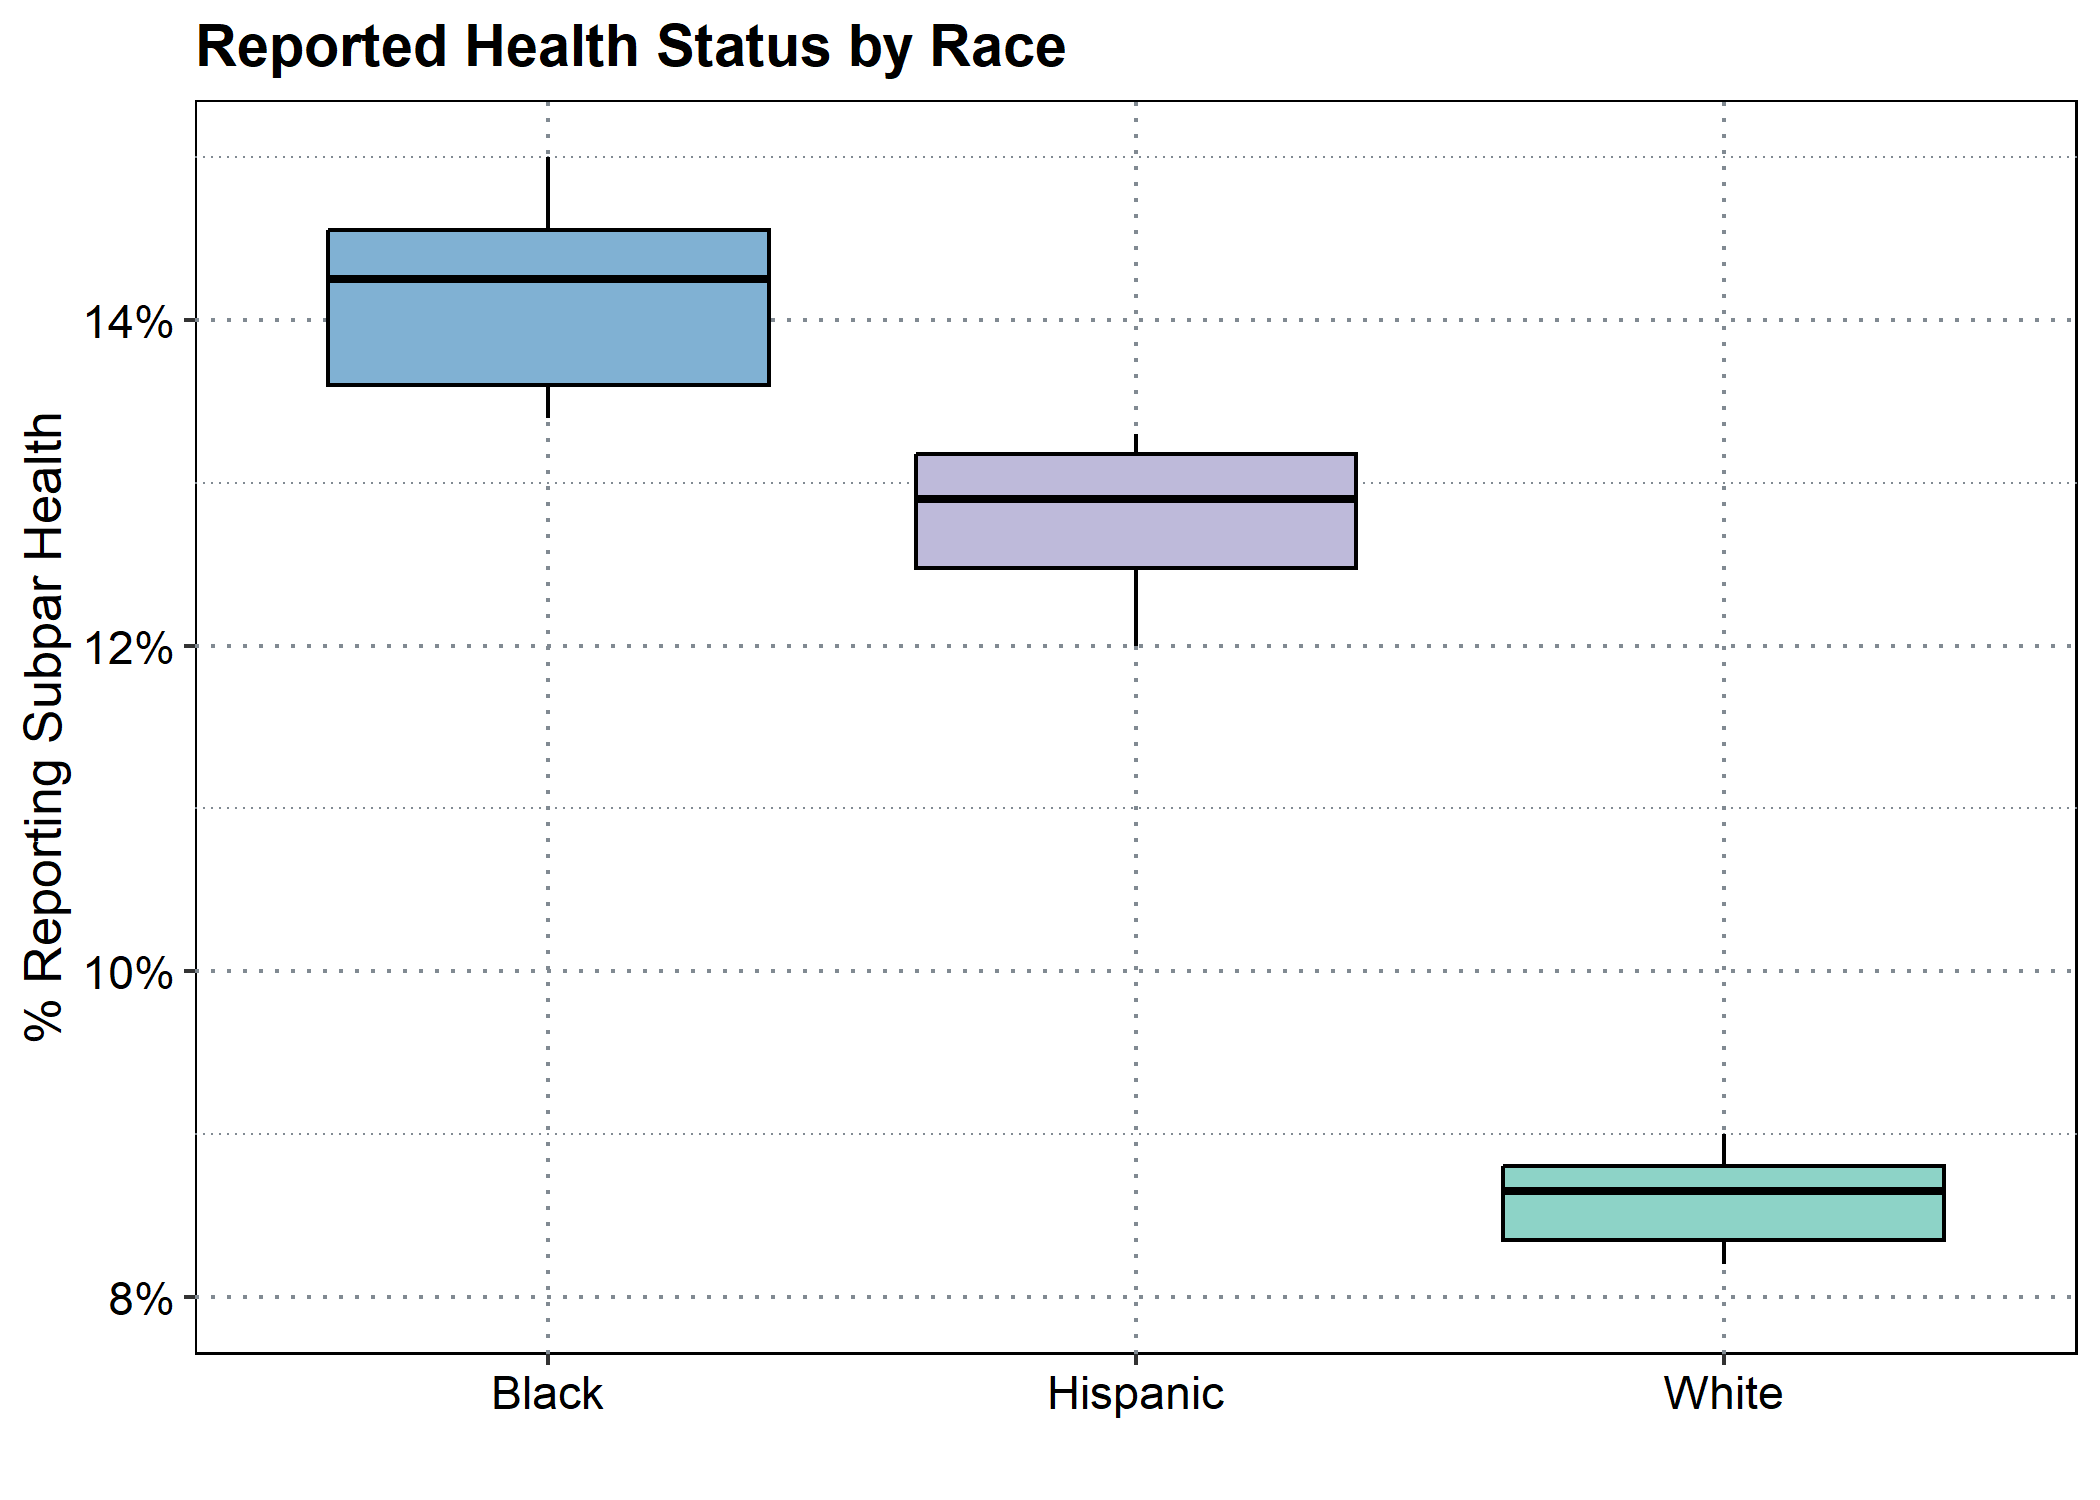
\includegraphics{Overview-Markdown_files/figure-latex/unnamed-chunk-8-1.pdf}

The following data trends will attempt to identify trends that may have
been driven by this leap upwards to 138\%.

First, let's look at trend in hospital visits:
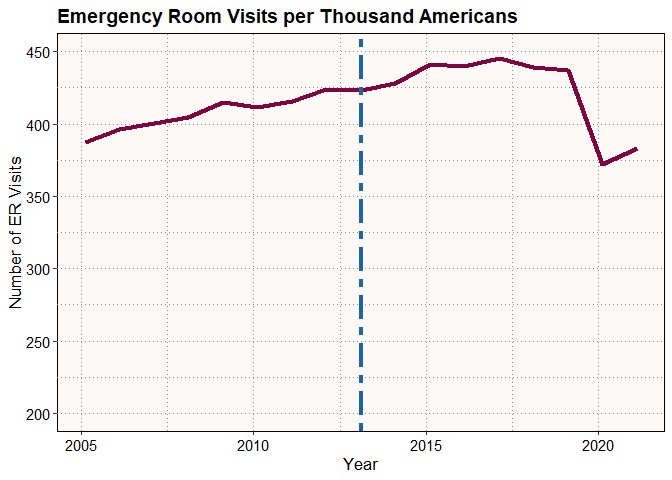
\includegraphics{Overview-Markdown_files/figure-latex/unnamed-chunk-9-1.pdf}

Then let's look at Americans foregoing medical care:
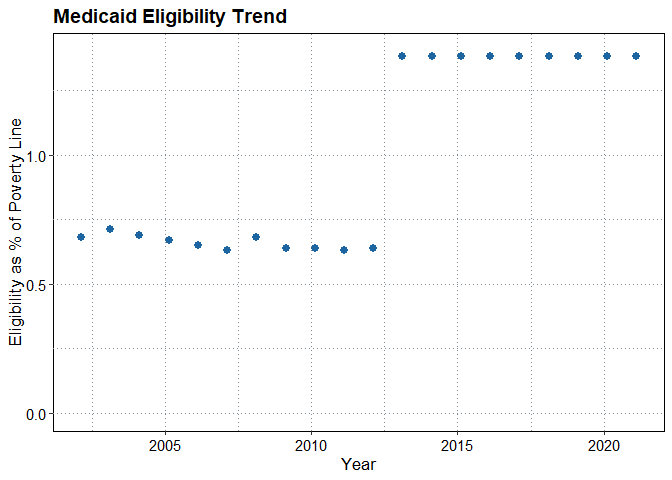
\includegraphics{Overview-Markdown_files/figure-latex/unnamed-chunk-10-1.pdf}

Next we'll look at assets and debts of the poorest Americans:
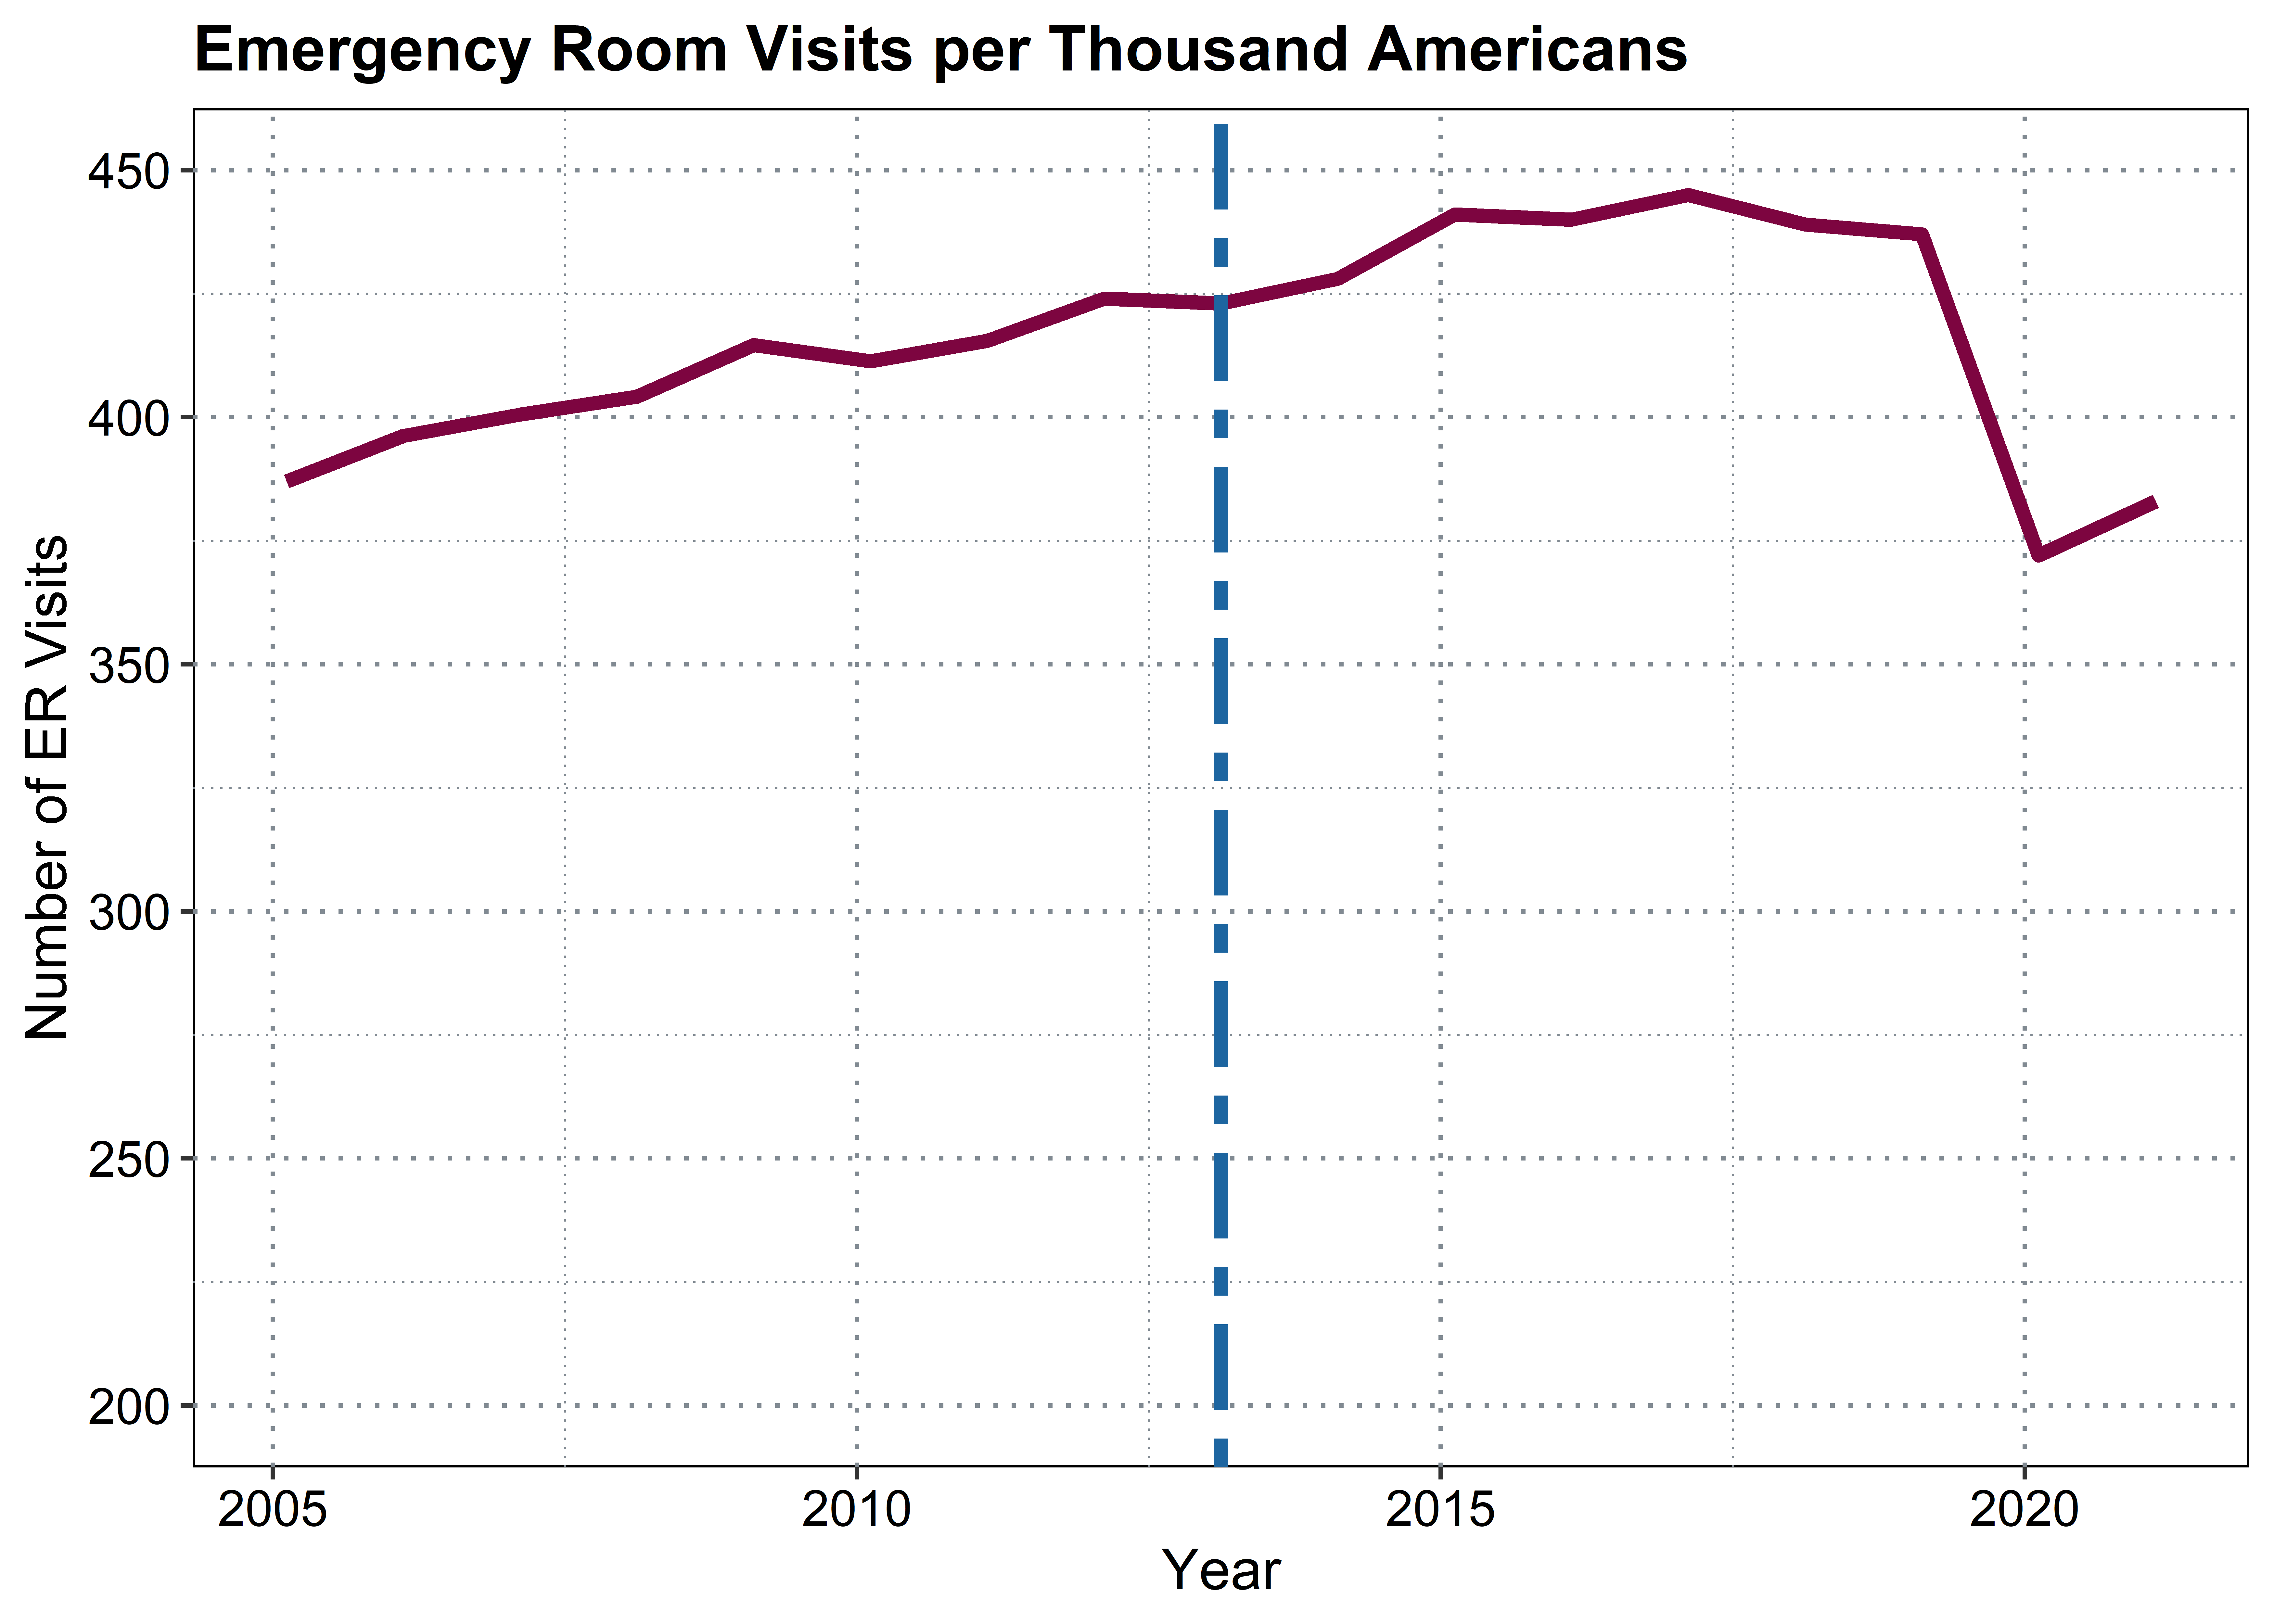
\includegraphics{Overview-Markdown_files/figure-latex/unnamed-chunk-11-1.pdf}

Health status of those under the poverty line:
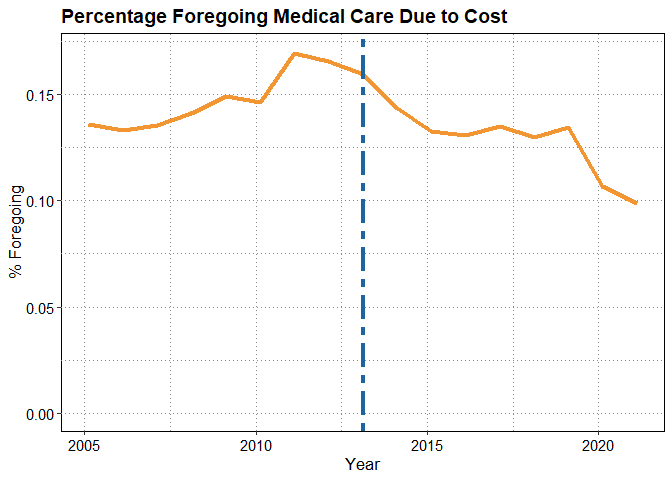
\includegraphics{Overview-Markdown_files/figure-latex/unnamed-chunk-12-1.pdf}

\end{document}
